\section{Improving GUI}
According to \cite{mchallenges} one of the challenges in mobile computing is small displays. Even though this article was written in 1994 and the size and resolution of mobile phones has increased greatly since then, it is still a challenge. While the a common laptop-computer has a 15 inch screen, the minimum requirement for an android phone is 2.5 inches and QVGA resolution (240 $\times$ 320 pixels). To cope with small screen sizes, the amount of elements in the user interface was reduced to a minimum, and buttons and lists made as large as possible. 
\subsection{Design principles}
\begin{quotation}
\emph{
The acronym KISS (Keep It Simple, Stupid) applies well to interface design. A simple, effective interface should be designed with the users' needs taking first priority.} \cite{guikisses}
\end{quotation}
\vspace{10 pt}
The user interface was designed following the ``KISS'' and ``Less is more'' principles. We wanted to keep it as basic as possible while still being aesthetically pleasing. Icons and symbols was not used as we wanted to have more space for text.

We chose to use colours from the Atb.no website, as these colours are associated with buses by people in Trondheim.
An early version of the GUI had buttons resembling the lcd signs found on the front of buses, but as the GUI for the rest of the application did not have a similar look, a more simplistic approach was preferred in the end. Contrasting colours were chosen to make text visible under various lighting conditions.

The suggestions in the original application was text based and used natural language. As we see it, this is not a very good solution for handheld devices with small screens, so these were redesigned to show the necessary information in minimal space, where intuitive graphics represented descriptions.

\begin{figure}
\begin{tabular}{ccc}
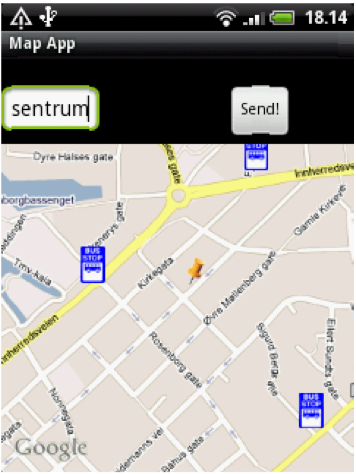
\includegraphics[width=0.33\linewidth]{DesigningGUI/magnus1.png} & 
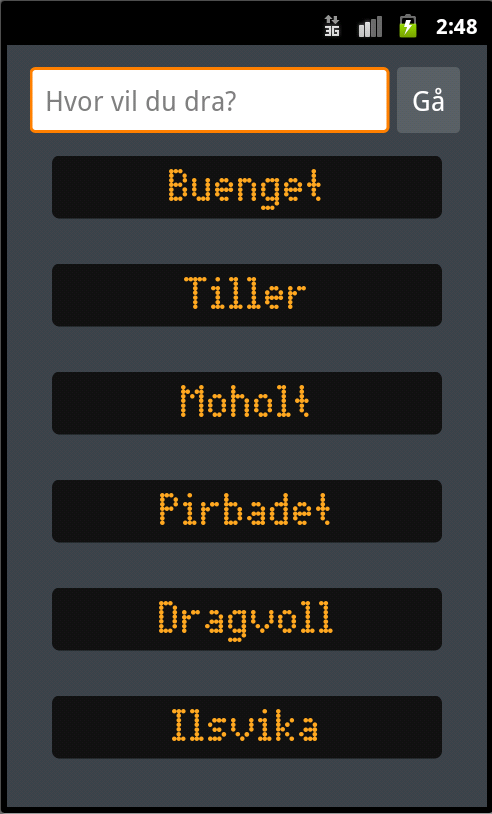
\includegraphics[width=0.33\linewidth]{DesigningGUI/earlydraft.png}&
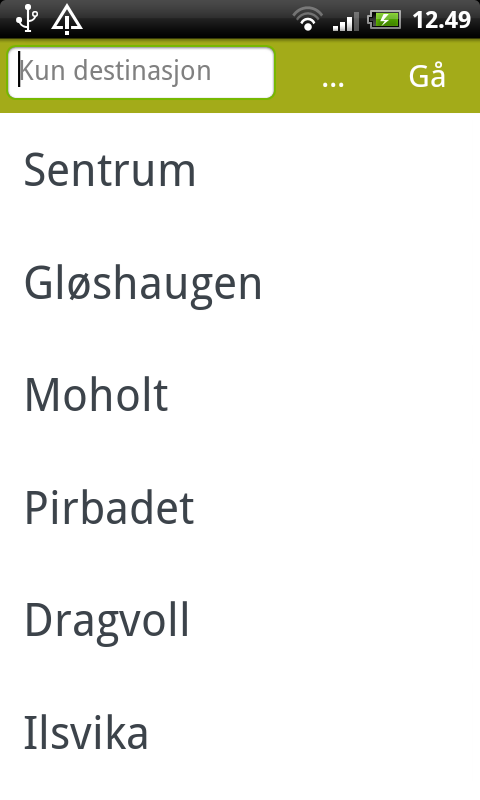
\includegraphics[width=0.33\linewidth]{DesigningGUI/finaldraft.png}
\end{tabular}
\caption{Raaum's home screen, First draft, Final draft}
\end{figure}
\begin{figure}
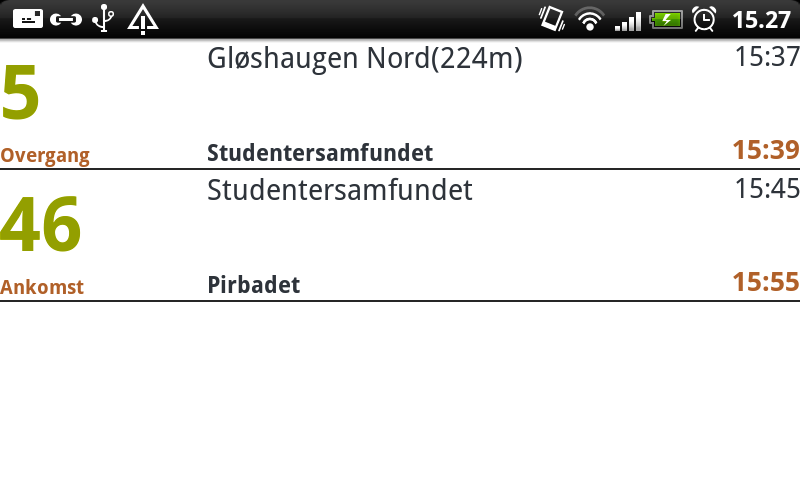
\includegraphics[width=1\linewidth]{DesigningGUI/suggestion.png}
\caption{The answer screen.}
\end{figure}
